\documentclass[12pt]{standalone}

\usepackage{tikz}

\begin{document}
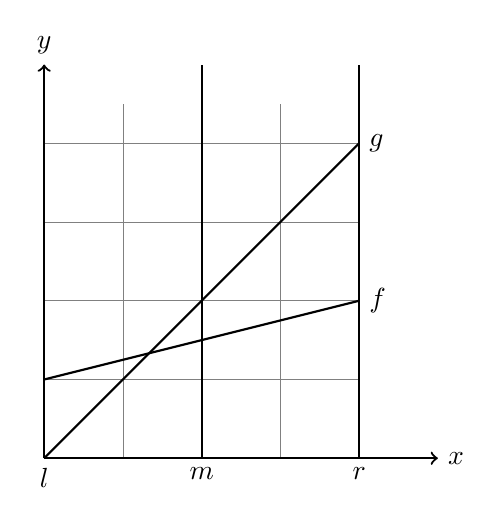
\begin{tikzpicture}

\draw[gray, very thin] (4,0) grid (0,4.5);

\draw[->,thick] (0,0) -- (0,5) node[above] {$y$};
\draw[->,thick] (0,0) -- (5,0) node[right] {$x$};

\node[below] at (0,0) {$l$};
\node[below] at (2,0) {$m$};
\node[below] at (4,0) {$r$};

\draw[thick] (2,0) -- (2,5);
\draw[thick] (4,0) -- (4,5);

\draw[thick] (0,1) -- (4,2) node[right] {$f$};
\draw[thick] (0,0) -- (4,4) node[right] {$g$};

\end{tikzpicture}
\end{document}
